%===============================================================================
% Template Projeto CDig - adaptado de SBAI/IFAC
% Relatorio ENE0167 Controle Digital 2026.1 - Processo Termico
% Template for IFAC meeting papers
% Copyright (c) 2007-2008 International Federation of Automatic Control
%===============================================================================
\documentclass[a4paper]{ifacconf}

\usepackage{xcolor}
\usepackage{graphicx,amsmath,url}      % include this line if your document contains figures
\usepackage[round]{natbib}             % required for bibliography
%===============================================================================


% ===============================================================
% Choose the language of the manuscript.
% If in English, choose
% \def\portugues{0}
%
% If in Portuguese or Spanish, choose
% \def\portugues{1}
\def\portugues{1}
% ===============================================================

% If the above line is commented, it is assumed manuscript in English:
\ifx\portugues\undefined
\def\portugues{0}
\fi


\if\portugues0
   \usepackage[english]{babel}
  \else
   \usepackage[spanish,brazil,english]{babel}
\fi



\usepackage[T1]{fontenc}
%\usepackage{inputenc}

\usepackage[utf8]{inputenc}

\usepackage{ae}


\if\portugues1
% =====================================================================
% If the manuscript is in Spanish, please change the texts adequatelly.
% =====================================================================
 \newtheorem{teorema}[thm]{{\em Teorema}}{ }
 \newtheorem{lema}[thm]{{\em Lema}}{ }
 \newtheorem{corolario}[thm]{{\em Corolário}}{ }
 \newenvironment{prova}{{\bf Prova.}}{ }
% ===============================================================
\fi

\begin{document}


\if\portugues1

% =====================================================================
% USE THIS PART IF THE TEXT IS IN PORTUGUES OR SPANISH
% =====================================================================
\selectlanguage{brazil}

\begin{frontmatter}

\collab{ENE0167 2026.1 Controle Digital - Prof. Adolfo Bauchspiess}

\title{Controle PI Anti-Windup Digital de Processo Térmico com Observador de Perturbações Senoidais}
% Title, preferably not more than 10 words.




\author[First]{José Henrique de L. Zeferino}
\author[Second]{Pedro Daniel B. Medeiros}

\address[First]{190125985, Engenharia Mecatrônica, UnB, jh.delucas@gmail.com}
\address[Second]{202028759, Engenharia Mecatrônica, pedrobomtempo2001@gmail.com}


\selectlanguage{english}
\renewcommand{\abstractname}{{\bf Abstract:~}}
\begin{abstract}                % Abstract of not more than 250 words.
\textit{This work presents the design and real-time implementation of a digital temperature
controller for a lumped-parameter thermal process actuated by PWM through an ESP32 micro\-controller.
A gray-box, two-pole/one-zero model with transport delay (P2DZ) is identified from an open-loop PRBS
experiment. An anti-windup PI controller is designed by the root-locus method to meet overshoot and
peak-time specifications, and is then extended, in the state space, with an augmented observer that
estimates and rejects the sinusoidal disturbance produced by a cooling fan. Continuous and discrete
simulations and experimental results obtained on the ESP32 are reported and compared.}

\vskip 1mm% não altere esse espaçamento
\selectlanguage{brazil}
{\noindent \bf Resumo}: Este relatório descreve o projeto e a implementação, em tempo real, de um sistema
de controle digital de temperatura. O processo térmico, a parâmetros concentrados, é aquecido por
resistores acionados em PWM por um microcontrolador ESP32 e perturbado por um ventilador. A partir de um
ensaio em malha aberta com sinal PRBS, identificou-se um modelo de dois polos, um zero e atraso de
transporte (P2DZ). Na primeira etapa (Prj1) projetou-se, via Lugar Geométrico das Raízes, um controlador
PI Anti-Windup discreto, atendendo às especificações de sobrepasso e tempo de pico e rejeitando
perturbações constantes por partes. Na segunda etapa (Prj2), manteve-se o canal PI e acrescentou-se,
no espaço de estados, um observador aumentado com modelo gerador de senoides, capaz de estimar e
rejeitar a perturbação senoidal do ventilador. Apresentam-se as simulações (contínua e discreta) e os
resultados experimentais coletados no ESP32, comparando-os com as especificações.
\end{abstract}

\selectlanguage{english}


\begin{keyword}
Digital control; Thermal process; System identification; PI Anti-Windup; Disturbance observer; State feedback.

\vskip 1mm% não altere esse espaçamento
\selectlanguage{brazil}
{\noindent\it Palavras-chaves:} Controle digital; Processo térmico; Identificação de sistemas; PI Anti-Windup; Observador de perturbações; Realimentação de estados.
\end{keyword}


\selectlanguage{brazil}


\end{frontmatter}
\else
% ===============================================================
% USE THIS PART IF THE TEXT IS IN ENGLISH (não utilizado)
% ===============================================================
\begin{frontmatter}
\title{Digital PI Anti-Windup Control of a Thermal Process}
\author[First]{First A. Author}
\address[First]{Universidade de Brasília}
\begin{abstract}
English version not used.
\end{abstract}
\begin{keyword}
Digital control; Thermal process.
\end{keyword}
\end{frontmatter}
\fi

%===============================================================================
%===============================================================================


\section{Introdução}

O controle de temperatura é um dos problemas mais recorrentes da engenharia de
automação, presente em processos industriais, em sistemas de climatização (HVAC) e em
equipamentos de laboratório. Processos térmicos são, em geral, lentos, dominados por uma
ou mais constantes de tempo e por um atraso de transporte associado ao deslocamento do
calor, o que os torna um excelente estudo de caso para técnicas de controle digital.

Este trabalho aborda o projeto e a implementação de um controlador digital para o
processo térmico didático da disciplina ENE0167, atuado por modulação por largura de
pulso (PWM) por meio de um microcontrolador ESP32. O trabalho divide-se em duas etapas
complementares: \textbf{Prj1}, o projeto de um controlador PI Anti-Windup discreto via Lugar
Geométrico das Raízes (LGR); e \textbf{Prj2}, a extensão do controle ao espaço de estados,
com um observador aumentado capaz de rejeitar perturbações senoidais geradas por um
ventilador. O modelo a parâmetros concentrados adotado segue os princípios fundamentais
de transferência de calor descritos em \cite{Bauchspiess:2006}.

\subsection{Objetivos}
\noindent \textbf{Geral:} projetar e implementar, em tempo real no ESP32, um sistema de
controle de temperatura que atenda a especificações dinâmicas e rejeite perturbações
constantes e senoidais.

\noindent \textbf{Específicos:} (i) identificar experimentalmente o modelo do processo;
(ii) projetar o PI Anti-Windup (Prj1) e o observador de perturbações senoidais (Prj2);
(iii) discretizar e embarcar os controladores; (iv) validar em simulação e experimentalmente.

\subsection{Especificações de Projeto}

As especificações seguem o grupo do roteiro \citep{Bauchspiess:CDig}, com ponto de operação
P.O.$\,=60\,^{\circ}$C e frequência da perturbação senoidal $\omega_0 = 0{,}098$~rad/s
(período $\approx 64$~s):

\textbf{Prj1 (PI Anti-Windup):}
\begin{itemize}
\item Sobrepasso $M_{p} \le 45\,\%$;
\item Tempo de pico $T_{p} = 30$~s;
\item Rejeição de perturbações constantes por partes;
\item Período de amostragem $T_s = 1$~s; resolução $\le 0{,}1\,^{\circ}$C.
\end{itemize}

\textbf{Prj2 (Observador Senoidal):}
\begin{itemize}
\item Resposta de 1\textsuperscript{a} ordem ($M_p = 0$);
\item Tempo de subida (10\%--90\%) $T_r = 30$~s;
\item Rejeição de perturbações constantes \emph{e} senoidais ($\omega_0$);
\item Período de amostragem $T_s = T_d$ (atraso medido no Prj1); resolução $\le 0{,}1\,^{\circ}$C.
\end{itemize}

%-------------------------------------------------------------------------
\section{Processo Térmico e Instrumentação}

O processo térmico, ilustrado na Figura~\ref{fig:circuito}, é constituído por um sensor de
temperatura LM35 aquecido por três resistores acionados em PWM através de um transistor
BC548. A variável controlada $y$ é a temperatura $T_p$ do conjunto sensor/resistores; a
variável manipulada $u$ é o \emph{duty-cycle} do PWM de aquecimento. Um segundo LM35 mede a
temperatura ambiente $T_a$, medida ``longe'' da perturbação. Um pequeno ventilador (\emph{cooler})
acionado por um segundo canal PWM resfria o processo, gerando perturbações constantes e
senoidais. Filtros RC passa-baixa, dimensionados conforme o \textit{datasheet} do
LM35 \citep{TI:LM35}, atenuam o ruído de medida; um amplificador de instrumentação pode
ajustar a faixa do sensor ($10\,$mV/$^{\circ}$C) à faixa do conversor A/D do ESP32 ($3{,}3$~V).

O modelo a parâmetros concentrados parte da capacitância térmica do conjunto e dos fluxos de
calor de aquecimento ($q_p$), do ambiente ($q_a$) e da perturbação ($q_w$), segundo a lei
$q_i = K_i (T_i - T)$ para condução/convecção \citep{Bauchspiess:2006}. Trata-se de um modelo
``caixa-cinza'', pois associa o polo rápido ao aquecimento PWM e o polo lento ao acoplamento
com $T_a$.

\begin{figure}[t]
 \begin{center}
  
\includegraphics[width=8.0cm]{figuras/resultados/foto_do_circuito.jpeg}
 \caption{Montagem experimental: \emph{protoboard} com ESP32 NodeMcu DevKit~v1, LM35,
 transistores BC548 e resistores de aquecimento; fonte de 12~V/1,5~A para o estágio de potência.}
 \label{fig:circuito}
 \end{center}
\end{figure}

\subsection{Materiais}
\textit{Protoboard}, ESP32 NodeMcu DevKit~v1 (chip USB--UART CP2102), 2$\times$LM35,
2$\times$BC548, \emph{cooler}, 3$\times$resistores ($\tfrac{1}{4}$~W) e filtro RC passa-baixa.
A comunicação com o PC é feita por USB; o \textit{driver} CP210x foi instalado para o
Windows~11 e a placa configurada no MATLAB como \texttt{ESP32-WROOM-DevKitV1}. Os sinais foram
coletados pelo software \emph{CoolTerm}. O acionamento usa os pinos D16 (aquecedor) e D17
(\emph{cooler}); as leituras, os pinos D13 ($T_p$) e D4 ($T_a$). Observou-se, na montagem, um
problema de \emph{sobrecorrente} em um dos BC548 ao acionar o \emph{cooler}, identificado após o
cálculo da corrente para o dimensionamento (em $\tfrac{1}{4}$~W) dos resistores.

%-------------------------------------------------------------------------
\section{Identificação do Modelo}

A obtenção dos parâmetros foi feita em malha aberta, em torno do ponto de operação, aplicando-se
um sinal binário pseudoaleatório (PRBS) ao aquecedor (firmware \texttt{CDigAquisicao.ino}; gerador
equivalente a \texttt{prbs.m}/\texttt{idinput}). O PRBS descorrelaciona a entrada dos parâmetros
estimados. Foram coletadas cerca de 6~horas de dados a $T_s = 1$~s (Figura~\ref{fig:prbs}),
registrando a temperatura diferencial $\Delta T = T_p - T_a$ e o \emph{duty-cycle}.

\begin{figure}[t]
 \begin{center}
  \includegraphics[width=8.4cm]{figuras/resultados/coleta_prbs.png}
 \caption{Ensaio de identificação em malha aberta: tensão do sensor de aquecimento (azul) sob
 excitação PRBS e temperatura ambiente (amarelo). Coleta de $\approx 6$~h a $T_s=1$~s.}
 \label{fig:prbs}
 \end{center}
\end{figure}

Após remoção das médias (\texttt{detrend}), a função \texttt{procest} estimou uma estrutura
\texttt{P2DZ} (dois polos, um zero e atraso), com o atraso travado em $T_d=5$~s, valor que
apresentou o melhor ajuste (\textit{fit}):
\begin{equation} \label{eq:proc}
\frac{Y(s)}{U(s)} = \frac{K_p\,(T_z s + 1)}{(T_{p1} s + 1)(T_{p2} s + 1)}\, e^{-T_d s}.
\end{equation}
Os parâmetros identificados são apresentados na Tabela~\ref{tab:modelo}. O polo rápido
($-1/T_{p2}$) está associado ao aquecimento PWM e o polo lento ($-1/T_{p1}$) ao acoplamento
com $T_a$.

\begin{table}[hb]
\begin{center}
\caption{Parâmetros do modelo P2DZ identificado.}\label{tab:modelo}
\begin{tabular}{cccccc}
\hline
$K_p$ & $T_{p1}$ [s] & $T_{p2}$ [s] & $T_z$ [s] & $T_d$ [s] \\ \hline
0,8864 & 323,16 & 37,636 & 278,32 & 5 \\ \hline
\end{tabular}
\end{center}
\end{table}

%-------------------------------------------------------------------------
\section{Prj1: Controle PI Anti-Windup}

\subsection{Projeto via LGR}
Adotou-se um controlador PI com a estrutura
\begin{equation} \label{eq:pi}
D(s) = K\,\frac{s + a}{s},
\end{equation}
projetada no Lugar Geométrico das Raízes com a ferramenta \emph{Control System Designer}
(\textsc{sisotool}). O atraso de transporte foi representado por uma aproximação de Padé de
1\textsuperscript{a} ordem, o que introduz um zero de fase não-mínima e impõe a redução do
ganho para preservar a estabilidade. Como o processo não é de 2\textsuperscript{a} ordem pura,
ajustou-se o sobrepasso para $\approx 35\,\%$ na ferramenta a fim de obter, na prática, os
$45\,\%$ especificados. Obteve-se $K = 3{,}25$ e $a = 0{,}106$, isto é,
$D(s) = 3{,}25\,(s+0{,}106)/s$ (Figura~\ref{fig:lgr}). A resposta ao degrau em malha fechada
(Figura~\ref{fig:resp}) confirma $M_p \approx 45\,\%$ e $T_p \approx 30{,}1$~s, atendendo às
especificações; a leve excursão negativa inicial deve-se ao zero de fase não-mínima
introduzido pela aproximação de Padé.

\begin{figure*}[t]
\begin{center}
    \includegraphics[width=0.44\linewidth]{figuras/resultados/LGR_Geogebra.jpeg}
    \hspace{0.02\linewidth}
    \fbox{\begin{minipage}[b]{0.44\linewidth}
    \centering \vspace{2.2cm}
    \textbf{[ESPAÇO RESERVADO]}\\[2mm]
    LGR do controlador PI plotado no MATLAB\\(Control System Designer) -- inserir figura.
    \vspace{2.2cm}
    \end{minipage}}
\end{center}
\caption{Projeto do PI no LGR. À esquerda, traçado no GeoGebra ($K_{\text{geo}}=0{,}3445$,
$A_{\text{geo}}=9{,}434$, com $a = 1/A_{\text{geo}}$ e $K = K_{\text{geo}}\,A_{\text{geo}}$);
à direita, espaço reservado para o LGR do MATLAB.}
\label{fig:lgr}
\end{figure*}

\begin{figure}[t]
 \begin{center}
  \includegraphics[width=8.0cm]{figuras/resultados/resp_temporal.jpeg}
 \caption{Resposta ao degrau, em malha fechada, do PI projetado (modelo com Padé). Pico em
 $t\approx 30{,}1$~s e amplitude $1{,}45$, ou seja, $M_p\approx 45\,\%$ e $T_p\approx 30$~s.}
 \label{fig:resp}
 \end{center}
\end{figure}

\subsection{Efeito Windup e Anti-Windup}
Todo atuador físico satura (aqui, o PWM é limitado entre $0$ e o valor de meia carga). Quando
o controlador com canal integral permanece saturado, o integrador acumula erro que não
corresponde à diferença entre referência e saída -- o fenômeno de \emph{windup} -- causando
sobrepasso e oscilações ao sair da saturação. Implementou-se um mecanismo \emph{anti-windup}:
o sinal é saturado \emph{antes} de atualizar a memória do integrador, de modo que apenas a
variação efetivamente aplicada ao \emph{hardware} é acumulada (cf.\ \texttt{CDigControle.ino}).

\subsection{Discretização}
O PI foi realizado de forma incremental (de velocidade):
\begin{equation} \label{eq:pidisc}
\Delta u[k] = q_0\, e[k] + q_1\, e[k-1] + \Delta u[k-1],
\end{equation}
com $u[k] = u_{\text{base}} + \Delta u[k]$. Compararam-se as discretizações de Tustin
($q_0=3{,}42225$, $q_1=-3{,}07775$) e de retentor de ordem zero (ZOH, $q_0=3{,}25$,
$q_1=-2{,}9055$); a versão ZOH apresentou menor oscilação na presença de perturbações e foi a
adotada. O firmware roda a $T_s = 1$~s, após um \emph{warm-up} de 4~min para levar o processo
ao P.O.

%-------------------------------------------------------------------------
\section{Prj2: Observador de Perturbações Senoidais}

Mantendo o canal PI do Prj1, o projeto foi reformulado no espaço de estados, acrescentando-se um
observador aumentado para estimar e rejeitar a perturbação senoidal do ventilador
(Figura~\ref{fig:bloco}). Da expansão modal de \eqref{eq:proc} obtém-se
\begin{equation}
A = \begin{bmatrix} -1/T_{p1} & 0\\ 0 & -1/T_{p2}\end{bmatrix},\;
B = \begin{bmatrix} K_p\\ K_p\end{bmatrix},\;
C = \begin{bmatrix} \alpha/T_{p1} & \beta/T_{p2}\end{bmatrix},
\end{equation}
com resíduos $\alpha = (T_z - T_{p1})/(T_{p2} - T_{p1}) \approx 0{,}157$ e $\beta = 1-\alpha$.

\subsection{Controlador aumentado (canal I)}
O sistema é aumentado com o estado integral $x_i$ e os polos são alocados por
\texttt{acker}. Aloca-se deliberadamente um polo \emph{sobre o zero} do processo, $-1/T_z$, e
o terceiro polo (do integrador) em $3\,p_1$, com $p = [-2{,}2/90,\; -1/T_z]$. Um fator de
ajuste de ganho $N_b = -K_i/p_1$ cancela um dos polos de malha fechada, mantendo a função de
transferência global de 1\textsuperscript{a} ordem (estrutura ``proporcional à referência,
integral do erro''), conforme a regra de Mason.

\subsection{Observador aumentado senoidal}
Ao observador do processo acrescenta-se o modelo gerador de senoides
\begin{equation}
A_s = \begin{bmatrix} 0 & 1\\ -\omega_0^2 & 0\end{bmatrix},\qquad \omega_0 = 0{,}098~\text{rad/s},
\end{equation}
resultando em um observador de 4\textsuperscript{a} ordem cujo ganho $L$ é obtido por
\texttt{acker} com polos $12\times$ mais rápidos que os do processo. A componente estimada da
senoide é então subtraída do sinal de controle, rejeitando a perturbação.

\subsection{Discretização e implementação}
O sistema aumentado foi discretizado por ZOH (\texttt{c2d}), com mapeamento exato dos polos
$z = e^{s T_s}$ e $T_s = T_d = 5$~s. O próprio \emph{script} \texttt{Prj2CDig\_m.m} gera as
matrizes discretas embarcadas no ESP32 ($A_d$ $4\times4$, $B_d$, $C_d$, $L_d$, ganho de
estados $K_d$, $K_{i,d}=19{,}59$ e $N_{b,d}=167{,}59$; cf.\ \texttt{CDigControle2.ino}). A
implementação usa PWM de 16~bits, saturação a meia carga, integração anti-windup condicional e
atualização do observador com o controle efetivamente aplicado.

\begin{figure*}[t]
\begin{center}
    
\includegraphics[width=0.92\linewidth]{figuras/resultados/diagrama_de_blocos_com_ZOH.jpeg}
\end{center}
\caption{Diagrama de blocos do Prj2 (Simulink): canal PI, observador do modelo do processo,
observador de perturbação senoidal e realimentação dos estados observados.}
\label{fig:bloco}
\end{figure*}

\begin{figure*}[t]
\begin{center}
    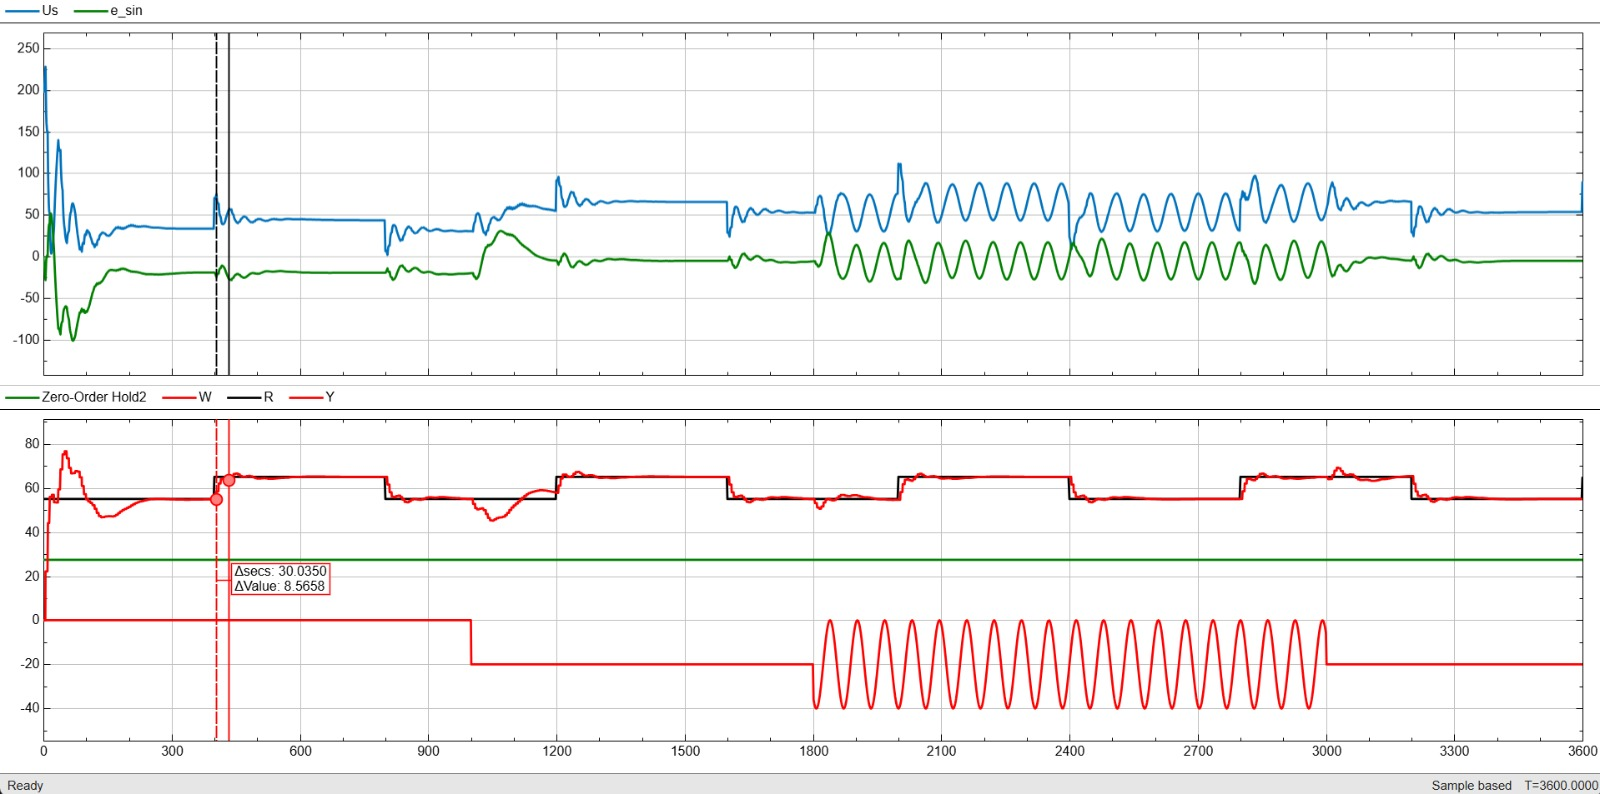
\includegraphics[width=0.92\linewidth]{figuras/resultados/resposta_sist_discretizado.jpeg}
\end{center}
\caption{Simulação do sistema discretizado (Prj2, $T_s=5$~s). A saída $Y$ (vermelho) segue a
referência $R$ (preto), rejeita o degrau de perturbação $W$ ($t\approx1000$~s) e a perturbação
senoidal ($t\approx1800$~s); medida $\Delta\text{secs}\approx30$~s confirma $T_r$.}
\label{fig:simdisc}
\end{figure*}

As simulações contínua e discreta validam o projeto: a versão discreta
(Figura~\ref{fig:simdisc}) cumpre $T_r \approx 30$~s e rejeita tanto o degrau quanto a senoide de
perturbação. Nota-se que o observador senoidal gera também uma componente DC, que se compõe com
a do canal PI.

%-------------------------------------------------------------------------
\section{Resultados Experimentais}

Os controladores foram embarcados no ESP32 e os sinais coletados em experimentos de
$\approx 1$~h, com varredura de degraus de $\pm 5\,^{\circ}$C em torno do P.O., perturbação
constante (meia carga do \emph{cooler}) e, por fim, perturbação senoidal.

\textbf{Prj1.} A Figura~\ref{fig:expprj1} mostra a saída e o sinal do \emph{cooler}/controle
para o PI Anti-Windup discretizado por ZOH. O sistema segue bem os degraus de referência e
rejeita a perturbação constante; sob perturbação senoidal, surge a oscilação residual esperada
de um PI (atenuação, não rejeição). A discretização por ZOH mostrou-se mais suave que a de
Tustin, que apresentou maior \emph{ringing}.

\begin{figure*}[t]
\begin{center}
    \includegraphics[width=0.80\linewidth]{figuras/resultados/y_abs_ctrl-ZOH.png}\\[1mm]
    \includegraphics[width=0.80\linewidth]{figuras/resultados/estado_cooler-ZOH.png}
\end{center}
\caption{Resultado experimental do Prj1 (PI Anti-Windup, ZOH). Acima: temperatura $y$ (azul) e
referência (vermelho). Abaixo: estado do \emph{cooler} (azul) e sinal de controle PWM (vermelho).}
\label{fig:expprj1}
\end{figure*}

\textbf{Prj2.} A Figura~\ref{fig:expprj2} apresenta o resultado do controle no espaço de estados
com observador senoidal. A saída segue a referência e rejeita o degrau de perturbação; durante a
perturbação senoidal (acionamento cíclico do \emph{cooler}), a oscilação da temperatura é
significativamente reduzida em relação ao Prj1, confirmando a ação do observador.

\begin{figure*}[t]
\begin{center}
    \includegraphics[width=0.92\linewidth]{figuras/resultados/coleta_prj2.png}
\end{center}
\caption{Resultado experimental do Prj2: temperatura $Y_{real}$ (azul), \emph{setpoint} (vermelho),
$T_a$ (amarelo) e estado do \emph{cooler} (verde, com perturbação senoidal na fase final).}
\label{fig:expprj2}
\end{figure*}

\begin{table}[hb]
\begin{center}
\caption{Especificações: projeto/simulação \emph{vs.} experimento.}\label{tab:comp}
\begin{tabular}{lccc}
\hline
 & Espec. & Simulação & Experim. \\ \hline
$M_p$ (Prj1) & $\le 45\,\%$ & $\approx 45\,\%$ & atendido \\
$T_p$ (Prj1) [s] & 30 & $\approx 30{,}1$ & $\approx 30$ \\
$T_r$ (Prj2) [s] & 30 & $\approx 30$ & $\approx 30$ \\
Rej.\ degrau & sim & sim & sim \\
Rej.\ senoide & sim & sim & atenuada \\ \hline
\end{tabular}
\end{center}
\end{table}

\subsection{Análise crítica}
O atraso de transporte de $\approx 5$~s foi o fator mais limitante do projeto: ele impõe perda de
fase e obriga a um compromisso entre rapidez e estabilidade, motivando o cancelamento de polos no
Prj2 e a escolha de $T_s = T_d$. A discretização ZOH superou a de Tustin na prática. As principais
fontes de discrepância entre simulação e experimento são a variação dos parâmetros térmicos com a
montagem, o ruído estocástico do processo a parâmetros distribuídos e as limitações do
\emph{hardware} (saturação restrita à meia carga para proteger os resistores e os transistores).

%-------------------------------------------------------------------------
\section{Conclusão}

Projetou-se e implementou-se, em tempo real no ESP32, um sistema de controle digital de
temperatura. A partir de um modelo P2DZ identificado por PRBS, o controlador PI Anti-Windup
(Prj1) atendeu às especificações de sobrepasso e tempo de pico e rejeitou perturbações
constantes. A reformulação no espaço de estados com observador aumentado (Prj2) permitiu também
a rejeição da perturbação senoidal, reduzindo de forma marcante a oscilação residual observada
no Prj1, com resposta global de 1\textsuperscript{a} ordem.

O trabalho evidenciou que a ferramenta computacional (LGR, Simulink, projeto no espaço de
estados) é indispensável, mas não substitui o entendimento dos conceitos: o tratamento do atraso
de transporte, a escolha do período de amostragem e o anti-windup foram decisivos para o
desempenho. Como extensões, citam-se o uso de um Preditor de Smith para o atraso e o refinamento
do modelo a parâmetros distribuídos. Os códigos e dados estão disponíveis no
repositório do projeto\footnote{\url{https://github.com/Joseph-deLZ/CDig_Prj}}.

\section*{Agradecimentos}
Os autores agradecem ao Prof.\ Adolfo Bauchspiess pela orientação e aos colegas da disciplina
ENE0167 pelas discussões.

\bibliography{OverleafCDig}             % bib file to produce the bibliography with bibtex

\end{document}
